\setcounter{mtc}{5} % real chapter number for the mini-TOC
\chapter{General Context and Analysis}
\minitoc

\graphicspath{{Chapter1/figures/}}
%==============================================================================
\pagestyle{fancy}
\fancyhf{}
\fancyhead[R]{\bfseries\chaptername~\thechapter.}
\fancyfoot[R]{\thepage}
\renewcommand{\headrulewidth}{0.5pt}
\renewcommand{\footrulewidth}{0pt}

\begin{spacing}{1.2}
%==============================================================================

\section*{Introduction}
% TODO: 1-2 paragraphs.
% State what this chapter covers (company + project context + requirements
% + methodology) and why it sits before the architectural chapter (Ch.II)
% and the release-based chapters (Ch.III onwards).
% The architectural narrative -- CQRS/ES, comby framework, domain model,
% deployment topology -- lives in Chapter II, NOT here. This chapter
% answers ``who, what, why, with what constraints''. Chapter II answers
% ``how, structurally''.

%--------------------------------------------------------------------
\section{Hosting company: Gradient Zero}
% TODO:
%   - General presentation (founded, mission, headquartered in Berlin/DACH).
%   - Activities and areas of expertise (data platforms, contract management,
%     custom CQRS/ES framework `comby`).
%   - The team I worked with (CTO, internal mentors).
%   - Where CLMPilot fits in the product portfolio.

\subsection{General presentation}
\dots

\subsection{Areas of expertise}
\dots

\subsection{Team and supervision}
\dots

%--------------------------------------------------------------------
\section{Project context: CLM in the DACH Mittelstand}
% TODO:
%   - The Mittelstand segment (100-5000 employees in DACH).
%   - Today's status quo: contracts in email, shared drives, file cabinets.
%   - Market size (~350k companies in DACH; 13\% CAGR globally).
%   - Compliance pressure (GoBD, GDPR, ISO 27001).
%   - Where existing players sit (SAP CLM / ServiceNow / Ironclad / Juro
%     / DACH niche players).
\dots

\subsection{The Mittelstand segment}
\dots

\subsection{Market and compliance pressure}
\dots

\subsection{Competitive landscape}
% Reuse the matrix from the project brief.
% Acceptable to put the comparison table here OR in Phase 2 (Custom fields)
% chapter. I keep it here because it motivates the project's scope choices.
\dots

%--------------------------------------------------------------------
\section{Problem statement}
% TODO: One paragraph per pain point, citing concrete numbers.
%   - Missed deadlines (auto-renewal triggers silently; thousands of EUR lost).
%   - No audit trail (GoBD/ISO 27001 failure).
%   - No portfolio overview (strategic decisions made blind).
%   - Approval chaos (no enforceable process).
\dots

%--------------------------------------------------------------------
\section{Functional requirements}
% TODO: Group by use case area; cite the actor that triggers each.
%   1. Contract registry (CRUD, search, filters).
%   2. Document linking (Google Drive / SharePoint / URL).
%   3. Deadline and renewal management (reminders at 90/60/30 days).
%   4. Approval workflows (configurable multi-step, audit trail).
%   5. Compliance audit trail (immutable, exportable).
%   6. Dashboard and reporting.
%   7. Identity & access (RBAC, MFA, password reset, invitations).

\subsection{Contract registry}
\dots

\subsection{Document linking}
\dots

\subsection{Deadline and renewal management}
\dots

\subsection{Approval workflows}
\dots

\subsection{Compliance and audit trail}
\dots

\subsection{Dashboard and reporting}
\dots

\subsection{Identity and access management}
\dots

%--------------------------------------------------------------------
\section{Non-functional requirements}
% TODO: Cover each NFR axis with one or two concrete constraints.
%   - Security (TLS 1.3, RBAC, MFA, encryption at rest).
%   - Compliance (GoBD, GDPR, EU data residency).
%   - Availability (target SLO; backup / DR window).
%   - Performance (page load, document linking latency).
%   - Auditability (every action immutable, time-stamped).
%   - Internationalisation (EN primary; DE/FR for DACH).
%   - Maintainability (single-developer-first; release train).

\subsection{Security}
\dots

\subsection{Compliance and data residency}
\dots

\subsection{Availability and reliability}
\dots

\subsection{Performance}
\dots

\subsection{Auditability}
\dots

\subsection{Internationalisation}
\dots

\subsection{Maintainability}
\dots

%--------------------------------------------------------------------
\section{Actors and high-level use cases}
% TODO: 1 use-case diagram + actor table.
%   Actors: Admin, Legal Manager, Approver, Auditor, External Reviewer (read-only).
%   Per the design rule (_Notes/design-and-diagrams.md): one diagram per actor
%   group when there are many use cases; don't dump everything into one box.

\subsection{Actor catalogue}
\dots

\subsection{Use-case diagram}
\begin{figure}[!ht]\centering
  % 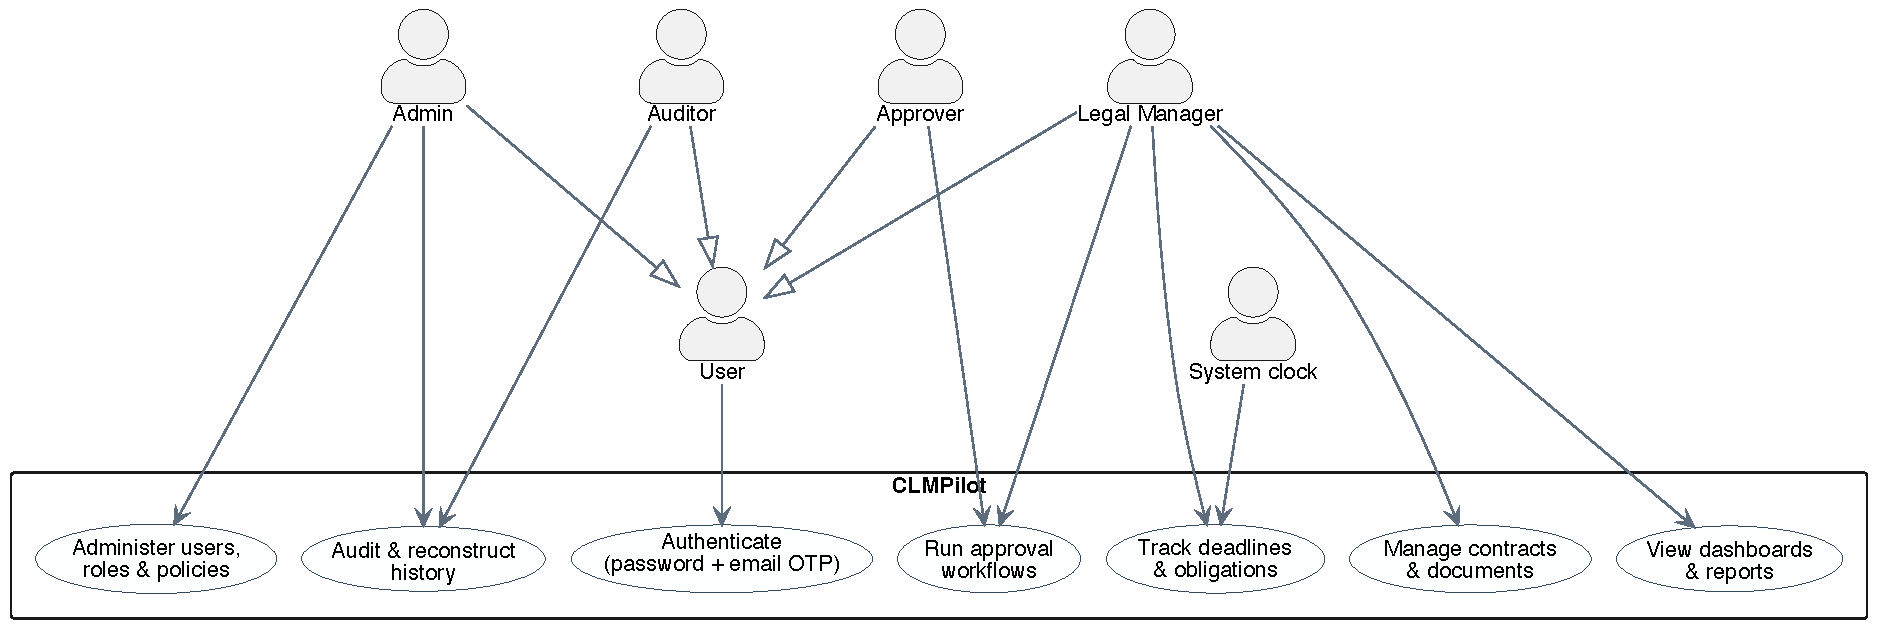
\includegraphics[scale=0.7]{usecase-overview.png}
  \caption{High-level use-case diagram for CLMPilot.}
  \label{fig:usecase}
\end{figure}

%--------------------------------------------------------------------
\section{Methodology}
% TODO: PROJECT-MANAGEMENT methodology only -- the architectural story
% lives in Chapter II.
%   - Release-train delivery model: explicit phase gates (Phase 0 -> 1A
%     -> 1B -> 1C -> Phase 2 -> Phase 3) with a milestone at each gate.
%   - Scrum-lite cadence: weekly planning, no fixed sprint length given
%     solo development; commit-level traceability via conventional
%     commits.
%   - Traceability: the roadmap is the single source of truth; chapter
%     numbering of THIS report mirrors the phase numbering of the
%     roadmap.
%   - Risk register and stakeholder communication via the auto-synced
%     Google Sheet.

\subsection{Release-train delivery}
\dots

\subsection{Planning cadence and traceability}
\dots

%--------------------------------------------------------------------
\section*{Conclusion}
% TODO: Recap (company + market + problem + requirements + methodology).
% Bridge to Chapter II: ``With the context and constraints set, the next
% chapter presents the architecture that addresses them, before the
% release-based chapters describe how that architecture was delivered.''
\dots

%==============================================================================
\end{spacing}
